\documentclass[../../../analisi-dei-requisiti.tex]{subfiles}

\begin{document}

\subsubsection{AUC10: Monitora dipendente}%
\label{subs:AUC10}

\begin{figure}[H]
  \centering
  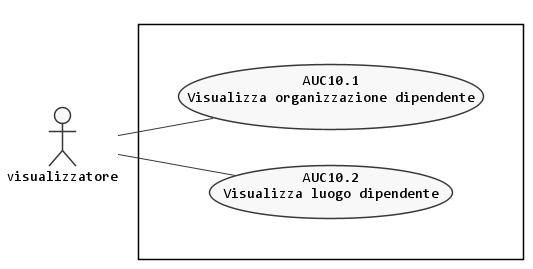
\includegraphics[width=100mm]{query-sul-dipendente.png}
  \caption{AUC10: Monitora dipendente}%
  \label{fig:AUC10}
\end{figure}

\begin{description}
  \item[Codice:] AUC10;
  \item[Titolo:] Monitora dipendente;
  \item[Attori primari:] visualizzatore;
  \item[Precondizione:]  il sistema deve rendere disponibile la pagina di monitoraggio dipendente;
  \item[Postcondizione:] il visualizzatore ottiene le informazioni di cui ha bisogno;
  \item[Scenario principale:]
  \begin{enumerate}
    \item il visualizzatore vuole ottenere delle informazioni riguardo ad un dipendente.
  \end{enumerate}
\end{description}

\end{document}

\subsubsection{AUC10.1: Visualizza organizzazione dipendente}%
\label{subs:AUC10.1}
\begin{description}
  \item[Codice:] AUC10.1;
  \item[Titolo:] Visualizza organizzazione dipendente;
  \item[Attori primari:] visualizzatore;
  \item[Precondizione:] il sistema risponde correttamente alle interrogazioni;
  \item[Postcondizione:] il visualizzatore conosce se il dipendente si trova nella/nelle organizzazioni su cui opera;
  \item[Scenario principale:]
  \begin{enumerate}
    \item il visualizzatore vuole sapere se il dipendente si trova all'interno di un'organizzazione in cui opera.
  \end{enumerate}
\end{description}

\subsubsection{AUC10.2: Visualizza luogo dipendente}%
\label{subs:AUC10.2}
\begin{description}
  \item[Codice:] AUC10.2;
  \item[Titolo:] Visualizza luogo dipendente;
  \item[Attori primari:] visualizzatore;
  \item[Precondizione:] il sistema risponde correttamente alle interrogazioni;
  \item[Postcondizione:] il visualizzatore conosce il luogo in cui si trova il dipendente;
  \item[Scenario principale:]
  \begin{enumerate}
    \item il visualizzatore vuole sapere in che luogo si trova un dipendente.
  \end{enumerate}
\end{description}
